% !TeX root = main.tex
% !TeX program = latexmk
\documentclass[11pt,a4paper]{report}

\usepackage[utf8]{inputenc}
\usepackage[T1]{fontenc}
\usepackage[dutch]{babel}
\usepackage{lmodern}
\usepackage{geometry}
\usepackage{setspace}
\usepackage{graphicx}
\usepackage{booktabs}
\usepackage{longtable}
\usepackage{array}
\usepackage{tabularx}
\usepackage{enumitem}
\usepackage{xcolor}
\usepackage{hyperref}
\usepackage{pdfpages}
\usepackage{titlesec}

\geometry{left=2.7cm,right=2.7cm,top=2.5cm,bottom=2.5cm}
%\onehalfspacing
\setlength{\parskip}{0.6em}
\setlength{\parindent}{0pt}
\emergencystretch=2em
\graphicspath{{figures/}}

\definecolor{pendingred}{RGB}{170,35,45}
\newcommand{\pending}[1]{%
  \par\noindent\fcolorbox{pendingred}{pendingred!8}{%
    \parbox[t]{0.94\textwidth}{\raggedright\textbf{NOG UIT TE VOEREN:} #1}}\par}
% detokenize makes file names such as lap_history.jsonl safe in normal text.
\newcommand{\code}[1]{\texttt{\detokenize{#1}}}

\hypersetup{
  colorlinks=true,
  linkcolor=black,
  citecolor=black,
  urlcolor=blue,
  pdftitle={Stageverslag Industriële Stage - Race Engineer Dashboard},
  pdfauthor={Jeff Mathieu}
}

\titleformat{\chapter}[display]
  {\normalfont\huge\bfseries}
  {\chaptertitlename\ \thechapter}{20pt}{\Huge}

\begin{document}

\pagenumbering{gobble}
\begin{titlepage}
  \centering
  \vspace*{2cm}
  {\Large KU Leuven\\Faculty of Engineering Science\\Master of Engineering: Computer Science\par}
  \vspace{2.5cm}
  {\Huge\bfseries Ontwikkeling van een live race-engineeringdashboard voor endurancewedstrijden\par}
  \vspace{2cm}
  {\Large Jeff Mathieu\par}
  \vfill
  \begin{tabular}{ll}
    Opleidingsonderdeel: & Industriële Stage: Computerwetenschappen \\
    Stageplaats: & MotorSport Training Center \\
    Dagelijkse begeleider: & Jan Wouters \\
    Stageperiode: & 22 juni -- 31 juli 2026 (zes weken) \\
    Academiejaar: & 2026--2027 \\
  \end{tabular}
  \vfill
  {\large \today\par}
\end{titlepage}

\pagenumbering{roman}
\chapter*{Abstract}
\addcontentsline{toc}{chapter}{Abstract}
Tijdens deze industriële stage van zes weken werd voor MotorSport Training Center een lokale desktopapplicatie ontwikkeld die live timingdata omzet in bruikbare informatie voor een race-engineer. De bestaande timingwebsites tonen de officiële rangschikking en actuele tijden, maar bieden niet alle teamgerichte vergelijkingen, voorspellingen en strategische hulpmiddelen die tijdens een endurancewedstrijd nodig zijn. De ontwikkelde Electron-applicatie leest daarom periodiek de timingpagina, normaliseert data van GetRaceResults en RIS Timing, bewaart de racehistoriek lokaal en berekent analyses buiten de gebruikersinterface.

Het resultaat is een dashboard voor maximaal drie gelijktijdig gevolgde wagens, met afzonderlijke modi voor race, kwalificatie en vrije training. Het systeem berekent onder andere ronde- en sectorgemiddelden, geldige beste tijden, voorspelde rondetijden, marges tegenover configureerbare referentietijden, vergelijkingen tussen piloten en klassewagens, inhaalindicaties en een pitstopplanning. Neutralisaties, pitgerelateerde rondes en onvolledige data worden expliciet behandeld. Een afzonderlijk grafiekvenster maakt langere trends zichtbaar. De data wordt per sessie opgeslagen in leesbare JSON-, JSONL- en CSV-bestanden, waardoor een sessie na een onderbreking kan worden hervat.

De ontwikkeling verliep iteratief en in nauw overleg met de opdrachtgever. Praktijktests en screenshots brachten verschillende subtiele fouten aan het licht, onder meer bij rondeachterstanden, intervalvelden, pitstopprojecties en wisselende timingproviders. Deze fouten leidden tot modulaire domeinfuncties en een uitgebreide automatische testsuite. Builds voor Windows en macOS worden via GitHub Actions gemaakt en als release gepubliceerd. De definitieve validatie tijdens de geplande test in Spa is op het moment van schrijven nog niet uitgevoerd en wordt daarom in dit verslag duidelijk als toekomstig werk aangeduid.

\textbf{Trefwoorden:} motorsport, live timing, Electron, race-engineering, rondetijdanalyse, pitstopstrategie, softwaretesten.

\chapter*{Administratieve gegevens}
\addcontentsline{toc}{chapter}{Administratieve gegevens}
\begin{tabularx}{\textwidth}{>{\bfseries\raggedright\arraybackslash}p{5.5cm}X}
Naam student & Jeff Mathieu \\
Opleiding & Master in de ingenieurswetenschappen: Computerwetenschappen \\
Stagebedrijf & MotorSport Training Center \\
Dagelijkse stagebegeleider & Jan Wouters \\
Contact begeleider & info@motorsport-trainingcenter.be \\
Stageperiode & 22 juni -- 31 juli 2026, zes weken \\
Opleidingsonderdeel & Industriële Stage: Computerwetenschappen \\
KU Leuven-coördinator & Prof. Tom Van Cutsem \\
\end{tabularx}

\tableofcontents
\clearpage
\pagenumbering{arabic}

\chapter{Inleiding en context}
\label{chap:context}

\section{Motorsport als beslissingsomgeving}
Een endurancewedstrijd is niet alleen een snelheidswedstrijd. Een team moet gedurende meerdere uren de prestaties van de wagen, verschillende piloten, concurrenten in dezelfde klasse, neutralisaties en verplichte pitstops opvolgen. Beslissingen worden genomen terwijl de wedstrijd blijft doorgaan. Informatie heeft daardoor alleen operationele waarde wanneer ze actueel, correct en snel interpreteerbaar is.

De publieke timingpagina is de primaire gegevensbron. Ze toont onder meer positie, klassepositie, wagen- en pilootinformatie, aantal ronden, laatste en beste rondetijd, sectortijden en verschillen tussen wagens. Deze tabel is ontworpen voor een algemeen publiek en voor het wedstrijdverloop als geheel. Een race-engineer stelt echter andere vragen: hoe verhoudt de huidige piloot zich tot zijn teamgenoot, hoe evolueert het tempo van de klasseleider, waar komt de wagen vermoedelijk uit na een pitstop, en nadert de voorspelde rondetijd een opgelegde referentietijd? Het voortdurend handmatig combineren van deze gegevens verhoogt de cognitieve belasting en de kans op rekenfouten.

\section{Stageplaats en opdracht}
De stage werd uitgevoerd voor MotorSport Training Center. De opdrachtgever bracht de motorsportkennis en de operationele verwachtingen aan; de technische analyse en implementatie gebeurden grotendeels zelfstandig. Hierdoor had de opdracht zowel het karakter van softwareontwikkeling als van technische consultancy. Een praktische vraag van de klant moest telkens worden omgezet in ondubbelzinnige gegevens, regels, algoritmes en schermcomponenten.

Het concrete doel was een desktopdashboard dat naast de officiële timingpagina kan draaien. De applicatie moest live data volgen, relevante historiek lokaal bewaren en de informatie specifiek voor het eigen team presenteren. De software moest bruikbaar zijn op Windows tijdens races, maar werd tijdens de stage hoofdzakelijk op macOS ontwikkeld. Platformonafhankelijkheid, eenvoudige installatie en herstel na een onderbreking waren daarom vanaf het begin belangrijke aandachtspunten.

\section{Doelstellingen}
De uiteindelijke opdracht bestond uit de volgende hoofddoelen:

\begin{itemize}
  \item live timingdata van meerdere websites betrouwbaar lezen en naar één intern formaat vertalen;
  \item een historiek van rondes, sectortijden en sessiecontext lokaal opslaan;
  \item maximaal drie wagens volgen zonder de timingwebsite drie keer te bevragen;
  \item analyses berekenen voor race, kwalificatie en vrije training;
  \item actuele rondevoorspellingen en configureerbare referentietijden tonen;
  \item een pitstopvenster en een projectie van de positie na een pitstop aanbieden;
  \item neutralisaties, pitstops, outlaps en onvolledige data correct behandelen;
  \item de logica modulair en automatisch testbaar maken;
  \item installaties en updates voor macOS en Windows via GitHub Releases ondersteunen.
\end{itemize}

\section{Afbakening}
De applicatie vervangt de officiële timing niet en neemt geen autonome strategische beslissingen. Ze gebruikt uitsluitend informatie die op de timingpagina beschikbaar is of vooraf door de gebruiker wordt geconfigureerd. Brandstofverbruik, bandentemperaturen, telemetrie uit de wagen en weersvoorspellingen maken geen deel uit van de huidige versie. De voorspellingen zijn beslissingsondersteuning en moeten altijd samen met de actuele wedstrijdcontext worden geïnterpreteerd.

Aanvankelijk werd ook gedacht aan replayfunctionaliteit en een uitgebreider machine-learningmodel. Tijdens de iteraties bleek dat betrouwbare live dataverwerking, uitlegbare berekeningen en racebestendige foutafhandeling meer waarde hadden binnen de beschikbare zes weken. Replayfunctionaliteit werd daarom uit de productieapp verwijderd. Voor tests werd wel een lokale simulator gebouwd op basis van historische wedstrijddata uit Assen. De rondevoorspelling gebruikt bewust een transparant model met recente sectorgemiddelden in plaats van een moeilijk uitlegbaar model.

\section{Leeswijzer}
Hoofdstuk~\ref{chap:requirements} beschrijft het iteratieve requirementsproces. Hoofdstuk~\ref{chap:architectuur} behandelt de softwarearchitectuur. Hoofdstukken~\ref{chap:data} en~\ref{chap:analyse} bespreken de dataverwerking en domeinlogica. Hoofdstuk~\ref{chap:interface} behandelt de interface. Daarna volgen verificatie en oplevering, de kritische reflectie en een afzonderlijk hoofdstuk met de nog uit te voeren validatie in Spa.

\chapter{Requirements en ontwikkelproces}
\label{chap:requirements}

\section{Iteratief overleg met de klant}
De requirements lagen bij de start niet volledig vast. De opdrachtgever wist welke informatie tijdens een race nodig was, maar de precieze voorstelling en rekenregels werden duidelijker door werkende versies te bekijken. Daarom werd gedurende de zes weken veelvuldig overlegd. Een typische iteratie bestond uit een vraag of schets van de klant, een eerste implementatie, een test met live of historische data en een bespreking van onverwacht gedrag.

Deze aanpak was noodzakelijk omdat ogenschijnlijk eenvoudige velden een domeinspecifieke betekenis hebben. Zo betekent \emph{DIFF} bij GetRaceResults het tijdsverschil met de vorige wagen in de algemene rangschikking, terwijl \emph{INT} bij RIS Timing een interval kan zijn dat in seconden of in ronden wordt uitgedrukt. Een kolom met de titel \emph{IN} bleek dan weer niet voor interval te staan, maar voor de ronde waarin de beste tijd werd gereden. Zulke verschillen kunnen alleen veilig worden verwerkt wanneer zowel de website als realistische wedstrijdsituaties worden onderzocht.

\section{Evolutie van de requirements}
De eerste dashboardversie bevatte een algemene sessiekaart, een klassentabel en grafieken. Feedback leidde tot een volledig hertekend scherm volgens een schets van de opdrachtgever. De informatie werd opgesplitst in grote tijdvakken, compacte sectorvakken, vergelijkingskolommen en een pitstopbalk. Later kwamen daar een donkere modus, een apart grafiekvenster en meerdere gelijktijdige dashboards bij.

Ook de achterliggende regels evolueerden. De oorspronkelijke referentietijdlogica werd eerst verwijderd omdat de betekenis van de regel nog niet voldoende duidelijk was. Nadat de gewenste werking was verduidelijkt, werd ze opnieuw toegevoegd als configureerbare lap- en sectorreferentie met kleurstatussen. De pitstopprojectie begon als een eenvoudige aftrek van de pitstoptijd. Tests toonden vervolgens dat rekening moest worden gehouden met alle tussenliggende wagens, ook uit andere klassen, met rondeachterstanden, providerafhankelijke intervallen en FCY-omstandigheden.

De opslagstrategie veranderde eveneens. Eerst werd automatisch een nieuwe map per start gemaakt. Dat was handig, maar onveilig wanneer de applicatie per ongeluk werd gesloten: een herstart zou een nieuwe sessie beginnen. De uiteindelijke keuze is dat de gebruiker zelf één map per sessie selecteert. Bij een herstart wordt bestaande JSONL-historiek geladen en worden alleen nieuwe ronden toegevoegd.

\section{Functionele vereisten}
De gerealiseerde functionele vereisten kunnen als volgt worden samengevat:

\begin{enumerate}[label=F\arabic*.]
  \item De gebruiker configureert timing-URL, sessiemodus, opslagmap en maximaal drie autonummers.
  \item De applicatie bevraagt de timingpagina om de vijf seconden en verdeelt dezelfde data over alle dashboards.
  \item De parser ondersteunt GetRaceResults en RIS Timing en bewaart de bronprovider.
  \item Voltooide ronden worden ontdubbeld en persistent opgeslagen.
  \item Race-, practice- en qualifyingmodus tonen aangepaste analyses.
  \item Rondes onder FCY, Safety Car of andere neutralisatie blijven opgeslagen maar worden uit representatieve tempoanalyses geweerd.
  \item Inlaps en outlaps blijven opgeslagen maar tellen niet mee voor tempovergelijkingen.
  \item Groene sectoren uit een gedeeltelijk geneutraliseerde ronde kunnen afzonderlijk geldig blijven, terwijl de volledige ronde ongeldig is voor het rondetijdgemiddelde.
  \item De voorspelde rondetijd gebruikt actuele sectoren en recente sectordata van de huidige piloot.
  \item De gebruiker kan lap- en sectorreferenties aanpassen en ziet de veiligheidsmarge via kleuren en delta's.
  \item De pitstopplanner houdt rekening met openingsvensters, cooldown, verplichte stops en een instelbare pitstoptijd.
  \item Grafieken tonen piloot-, sector- en klassevergelijkingen en ondersteunen zoomen bij lange reeksen.
  \item De app kan na een crash of sluiting verdergaan vanuit dezelfde sessiemap.
\end{enumerate}

\section{Niet-functionele vereisten}
Tijdens een race wegen betrouwbaarheid en begrijpelijkheid zwaarder dan theoretische complexiteit. De berekeningen moesten daarom deterministisch, uitlegbaar en onafhankelijk van de renderer zijn. De renderer krijgt kant-en-klare viewmodellen en formatteert of berekent geen racebeslissingen zelf. Elke belangrijke domeinfunctie moest met synthetische en historische data testbaar zijn.

Verder moest de applicatie langdurig kunnen draaien zonder onbegrensde geheugengroei of overmatige opslag. De pollingfrequentie van vijf seconden levert tijdens 24 uur 17.280 meetmomenten op, maar alleen gewijzigde snapshots en voltooide rondes worden als relevante historiek bewaard. Het gebruik van één collector voor maximaal drie dashboards voorkomt onnodige netwerkbelasting.

\section{Planning over zes weken}
De uitvoering verliep niet als zes strikt gescheiden fasen. In de eerste periode lag de nadruk op parser, live collector en opslag. Daarna volgden dashboardanalyse, tests en de nieuwe UI. Pitstoplogica, voorspelling, sessiemodi en grafieken werden in opeenvolgende iteraties toegevoegd. In de laatste fase kwamen provideredgecases, FCY-projecties, distributie, automatische updates en herstel na herstart aan bod.

Deze iteratieve volgorde week af van een klassiek vooraf vastgelegd stageplan, maar paste beter bij de beschikbaarheid van live demo's en klantfeedback. Bugs die alleen in een bijna volledige race zichtbaar werden, hadden een grotere impact op de prioriteiten dan oorspronkelijk geplande uitbreidingen.


\chapter{Technische architectuur}
\label{chap:architectuur}

\section{Electron als desktopplatform}
De applicatie is gebouwd met Electron en JavaScript. Electron combineert een Chromium-renderer met een Node.js-mainproces. Deze keuze maakte het mogelijk om een webgebaseerde interface te bouwen en tegelijk lokale bestanden, native dialoogvensters en meerdere desktopvensters te beheren. Dezelfde codebasis kan voor macOS en Windows worden verpakt.

Het mainproces in \code{src/main/main.js} beheert de levenscyclus van de applicatie, instellingen, vensters, polling, opslag en IPC-handlers. Het verborgen livevenster laadt de echte timingwebsite. Een extractiescript wordt in die pagina uitgevoerd om tabelkoppen, cellen en sessie-informatie uit de gerenderde DOM te lezen. Hierdoor kan de applicatie ook dynamische websites verwerken die niet als eenvoudige statische HTML beschikbaar zijn.

\section{Proces- en modulegrenzen}
De code is bewust in drie zones verdeeld:

\begin{itemize}
  \item \code{src/main}: Electron-specifieke infrastructuur, vensters, updates en bestands-I/O;
  \item \code{src/shared}: pure domeinfuncties voor parsing, analyse, voorspelling, pitstops en viewmodellen;
  \item \code{src/renderer}: HTML, CSS en code die reeds berekende data op het scherm zet.
\end{itemize}

De preloadlaag vormt de gecontroleerde brug tussen renderer en mainproces. \code{contextIsolation} staat aan en \code{nodeIntegration} uit, zodat de renderer niet rechtstreeks toegang krijgt tot Node.js. Alleen expliciet aangeboden functies, zoals instellingen ophalen, collectie starten of een grafiekvenster openen, zijn beschikbaar.

De scheiding tussen renderer en domeinlogica was een belangrijke verbetering tijdens de stage. Vroege versies bevatten berekeningen in de UI-code. Daardoor was het moeilijk om te bewijzen dat een waarde correct was en konden verschillende schermen dezelfde berekening anders uitvoeren. In de huidige architectuur leveren modules zoals \code{lapAnalytics.js}, \code{classBattle.js}, \code{lapPrediction.js} en \code{pitstopPlanner.js} volledige resultaten. De renderer beperkt zich tot selectie, presentatie en gebruikersinteractie.

\section{Vensterarchitectuur}
Er is één hoofdvenster voor de primaire wagen. Wanneer de gebruiker via de setup een tweede of derde wagen toevoegt, opent voor elke extra wagen een dashboardvenster met dezelfde renderer en een andere wagenparameter. Alle vensters ontvangen dezelfde collectorstatus. De timingwebsite wordt dus slechts eenmaal geladen en bevraagd.

Grafieken worden in afzonderlijke vensters geopend. Ook zij gebruiken de reeds opgeslagen lap history en starten geen eigen collector. Deze aanpak houdt het hoofdscherm compact en maakt het mogelijk om analysevensters alleen te openen wanneer ze nodig zijn.

Een verborgen BrowserWindow blijft tijdens collectie actief. Wanneer de gebruiker de timingpagina ter debugging toont en daarna sluit, wordt dit venster normaal verborgen in plaats van vernietigd. De algemene applicatielifecycle vormt daarop een uitzondering: bij een echte Quit worden polling en close-to-hide uitgeschakeld. Deze aparte lifecyclemodule lost een macOS-probleem op waarbij de app anders in de Dock actief bleef en alleen met Force Quit kon worden beëindigd.

\section{Datastroom}
Elke poll doorloopt dezelfde keten:

\begin{enumerate}
  \item Het extractiescript leest tabellen en sessievelden uit de livepagina.
  \item De parser herkent bruikbare headers en zet elke rij om naar canonieke velden.
  \item De storage-normalizer voegt provider- en sessiecontext toe.
  \item Nieuwe voltooide ronden worden via een stabiele identiteit ontdubbeld.
  \item De lap history en actuele rijen worden aan de analysemodules doorgegeven.
  \item Voor elke gevolgde wagen worden dashboardanalyse, voorspelling en pitstopplan berekend.
  \item De volledige collectorstatus wordt opgeslagen en via IPC naar alle vensters gestuurd.
\end{enumerate}

De UI en de berekeningen worden dus gevoed door dezelfde consistente snapshot. Dit voorkomt dat een grafiek bijvoorbeeld met gegevens van een andere poll rekent dan het hoofdscherm.

\section{Instellingen en configuratie}
Instellingen worden als JSON in de Electron user-datafolder bewaard. Ze omvatten timing-URL, gevolgde wagens, modus, thema, opslagmap, referentietijden en pitstopregels. Referentietijden zijn afzonderlijk per sessiemodus opgeslagen, zodat een qualifyingreferentie een racereferentie niet overschrijft. Circuitprofielen voor Spa, Zolder en Assen bevatten standaardwaarden voor de relevante afstand en FCY-snelheid. In de pitstopsetup kunnen deze waarden per evenement worden overschreven wanneer het reglement afwijkt.

\section{Bewuste technische beperkingen}
De timingwebsite blijft een externe afhankelijkheid. Een wijziging van DOM-structuur of kolomnamen kan parseraanpassingen vereisen. Daarom bewaart de applicatie parserdiagnostiek en blijft de livepagina zichtbaar via een debugactie. Ook worden onbekende of onbetrouwbare waarden niet stilzwijgend als nul geïnterpreteerd: analysefuncties retourneren waar mogelijk een expliciete onbeschikbare toestand.


\chapter{Afweging van alternatieve oplossingen}
\label{chap:alternatieven}

\section{Desktopapplicatie tegenover webapplicatie}
Een centrale webapplicatie was een mogelijk alternatief voor Electron. Een webserver zou updates voor alle gebruikers onmiddellijk beschikbaar maken en meerdere clients kunnen bedienen. Daartegenover staan extra operationele afhankelijkheden: hosting, authenticatie, netwerkconfiguratie en bereikbaarheid van de server. De timingbron is zelf al afhankelijk van internet. Door verwerking en opslag lokaal te houden wordt ten minste de reeds ontvangen historiek niet van een tweede externe dienst afhankelijk.

Een gewone lokale webserver met browserinterface had eveneens gekund. Electron voegt pakketgrootte en geheugengebruik toe, maar vereenvoudigt native bestandskeuze, vensterbeheer, installatie en distributie. Vooral het openen van afzonderlijke dashboards voor extra wagens en grafieken past goed bij een desktopapplicatie. Voor dit prototype woog die ontwikkelsnelheid zwaarder dan de grotere runtime.

Een volledig native Windowsapplicatie, bijvoorbeeld in C\#, zou een kleinere en nauwer geïntegreerde productieapp kunnen opleveren. De ontwikkeling gebeurde echter op macOS en het resultaat moest ook daar testbaar blijven. Electron maakte één gedeelde implementatie mogelijk. Wanneer de applicatie later zeer breed wordt uitgerold en resourcegebruik problematisch blijkt, kan een native frontend opnieuw worden onderzocht terwijl de pure domeinregels als specificatie behouden blijven.

\section{DOM-extractie tegenover een officiële API}
Een officiële JSON- of WebSocket-API zou betrouwbaarder zijn dan DOM-extractie. Velden zouden een gedocumenteerd type en vaste semantiek kunnen hebben. Voor de gebruikte publieke timingpagina's was zo'n uniforme beschikbare API niet het uitgangspunt. De applicatie leest daarom de gerenderde tabel die ook de gebruiker ziet.

Deze oplossing is pragmatisch maar kwetsbaar voor HTML-wijzigingen. De impact wordt beperkt door headercanonicalisatie, providerdetectie en parserdiagnostiek. Wanneer in de toekomst toegang tot een officiële feed beschikbaar wordt, kan een nieuwe collectoradapter worden toegevoegd. De downstreammodules hoeven dan niet te veranderen zolang dezelfde genormaliseerde rijen worden geproduceerd.

\section{Bestanden tegenover SQLite}
SQLite was aanvankelijk de voor de hand liggende keuze. Het biedt transacties, indexes en krachtige queries zonder afzonderlijke server. Voor de uiteindelijke schaal bleken bestanden echter voordelen te hebben. Een engineer kan een CSV direct openen, JSONL kan append-only worden geschreven en een beschadigde laatste regel tast niet noodzakelijk de volledige historiek aan. Ook export en debugging zijn eenvoudiger.

Het nadeel is dat relaties en constraints in applicatiecode worden bewaakt. Queries over meerdere grote evenementen zijn minder efficiënt. Wanneer later een centraal archief met vele races en interactieve historische analyses nodig is, wordt SQLite of PostgreSQL relevanter. De huidige storage schema-module biedt daarvoor al een uniforme representatie; migratie hoeft niet vanuit willekeurige rendererdata te gebeuren.

\section{Volledig incrementele tegenover herberekende statistiek}
Een gemiddelde kan efficiënt worden bijgewerkt met een teller en som. Voor een lange race lijkt dit aantrekkelijk. In dit project zijn ronden echter niet altijd definitief geldig op het eerste moment dat ze verschijnen. Pitstatus, sectorvlaggen of correcties kunnen de selectie beïnvloeden. Een gecachet gemiddelde zou dan teruggedraaid moeten worden met exact dezelfde eerdere context.

Daarom wordt de lap history als bron gebruikt en worden statistieken opnieuw uit de gefilterde relevante ronden berekend. Met enkele duizenden records en pure JavaScriptfuncties blijft dit snel genoeg. De laatst berekende samenvatting wordt wel opgeslagen voor inspectie. Pas wanneer metingen aantonen dat herberekenen een werkelijk prestatieprobleem vormt, is een incrementele cache met invalidatieregels verantwoord.

\section{Eenvoudige voorspelling tegenover machine learning}
Een regressiemodel, random forest of neuraal netwerk zou meerdere features kunnen combineren: piloot, bandenslijtage, brandstofniveau, verkeer, temperatuur en weersomstandigheden. De timingpagina levert veel van die inputs niet. De beschikbare trainingsdata is bovendien beperkt en bevat veranderende circuits en omstandigheden. Een complex model zou daardoor snel overfitten en moeilijk uitlegbaar zijn.

Het sectorgemiddeldenmodel heeft duidelijke beperkingen, maar iedere component kan op het dashboard worden verklaard. Het model reageert op actuele sectoren en gebruikt alleen recente data van dezelfde piloot. Een toekomstige uitbreiding kan deze baseline vergelijken met exponentiële weging of regressie. Een complexer model is pas zinvol wanneer het op historische sessies aantoonbaar een lagere fout heeft en zijn onzekerheid operationeel kan communiceren.

\section{Automatische tegenover handmatige modusdetectie}
De sessienaam bevat vaak woorden als Race, Qualifying of Practice. Automatische detectie lijkt dus eenvoudig. Toch verschillen talen, afkortingen en providerlabels, en een organisator kan een afwijkende naam gebruiken. Een fout gedetecteerde modus kan pitinformatie verbergen of verkeerde vergelijkingen tonen. Daarom kiest de gebruiker de modus expliciet. De extra handeling is klein en het gedrag blijft voorspelbaar.

\section{Iteratieve tegenover vooraf vastgelegde ontwikkeling}
Een watervalaanpak met een volledige specificatie vóór implementatie zou minder herwerking beloven. In deze opdracht bestond veel kennis echter impliciet bij de opdrachtgever. Pas een zichtbaar dashboard maakte duidelijk welke informatie ontbrak. Een iteratieve aanpak met korte feedbacklussen was daardoor geschikter.

Dit betekende niet dat elke nieuwe wens onmiddellijk zonder afweging werd toegevoegd. De architectuur werd gaandeweg strenger: gedeelde logica moest naar pure modules, nieuwe edgecases kregen regressietests en providerafhankelijke aannames moesten expliciet worden benoemd. Zo bleef het prototype ondanks veranderende requirements onderhoudbaar.


\chapter{Dataverwerking en lokale opslag}
\label{chap:data}

\section{Uniforme parser}
De timingproviders gebruiken verschillende labels en representaties. De parser begint daarom met het opschonen van witruimte en het canoniseren van headers. Varianten worden gekoppeld aan interne sleutels voor positie, startnummer, klasse, PIC, team, piloot, aantal ronden, gap, interval, sectoren, laatste tijd, beste tijd en pitinformatie. Een headercontrole voorkomt dat een willekeurige tabel op de pagina als timingtabel wordt gebruikt.

Tijdswaarden worden zo vroeg mogelijk naar milliseconden omgezet. De tekst \code{2:05.073} wordt intern bijvoorbeeld 125.073 milliseconden. Formatteringsfuncties zetten dit pas bij presentatie opnieuw om. Dit maakt optellen, middelen, vergelijken en testen eenduidig.

Elke genormaliseerde rij bevat ook de gedetecteerde bronprovider. Dat is noodzakelijk omdat een identiek ogend veld een andere semantiek kan hebben. GetRaceResults levert een bruikbare \emph{DIFF} tussen opeenvolgende algemene posities. Om de afstand tussen twee klassewagens te bepalen worden alle tussenliggende DIFF-waarden opgeteld, ook die van wagens uit een andere klasse. RIS Timing gebruikt \emph{INT}; wanneer die waarde een ronde-eenheid bevat, wordt de rondeachterstand conservatief omgerekend met een representatieve gemiddelde rondetijd. De code bevat daarnaast fallbacks voor onvolledige feeds.

\section{Detectie van voltooide ronden}
De live tabel bevat zowel de laatst voltooide rondetijd als sectoren van de ronde die bezig is. Bij elke poll wordt de laatste bekende rij per wagen bewaard. Wanneer de combinatie van wagen, ronde en tijd een nieuwe voltooide ronde aanduidt, wordt een laprecord gemaakt. De sectorwaarden van de vorige snapshot vormen dan het beste bewijs voor de sectoren van die voltooide ronde.

Een lap identity voorkomt duplicaten wanneer dezelfde live rij gedurende meerdere polls zichtbaar blijft. Bij een herstart worden identities uit de bestaande JSONL-historiek opnieuw in een set geladen. Nieuwe data kan daardoor veilig aan dezelfde sessie worden toegevoegd zonder oude ronden opnieuw te schrijven.

\section{Vlagstatus en pitfasen}
Voor elke sector wordt de vlagstatus vastgelegd op het moment dat de sector beschikbaar wordt. Dit detail is nodig voor het scenario waarin sector 1 groen wordt gereden en tijdens sector 2 FCY begint. De volledige ronde is dan niet representatief voor een rondetijdgemiddelde, maar sector 1 kan nog geldig zijn voor het gemiddelde en de beste waarde van sector 1.

De analyselaag annoteert ook pitfasen. Veranderingen in pitteller en pitstatus helpen inlaps en outlaps identificeren. Deze ronden blijven deel van de historische werkelijkheid, maar worden niet gebruikt voor representatief tempo. Dit voorkomt dat een trage pitronde het gemiddelde van een piloot kunstmatig verslechtert.

\section{Bestandsformaat}
Er werd uiteindelijk niet voor SQLite gekozen. Voor de schaal van één race en de behoefte aan inspecteerbaarheid bleken leesbare bestanden eenvoudiger en voldoende. De belangrijkste bestanden zijn:

\begin{itemize}
  \item \code{lap_history.jsonl}: append-only historiek met één JSON-object per ronde;
  \item \code{lap_history.csv}: tabelvorm voor manuele inspectie of spreadsheetanalyse;
  \item \code{latest_live_rows.json} en \code{.csv}: laatste volledige timingsnapshot;
  \item \code{session_metadata.json}: sessiecontext;
  \item \code{parser_debug.json}: gedetecteerde headers, voorbeelden en waarschuwingen;
  \item \code{analytics_summary.json}: laatst berekende statistieken;
  \item aparte prediction- en pitstopplanbestanden per gevolgde wagen.
\end{itemize}

JSONL is geschikt voor rondes omdat een nieuwe ronde kan worden toegevoegd zonder het volledige bestand te herschrijven. Tegelijk blijft elke regel leesbaar en herstelbaar. Samenvattingsbestanden worden wel overschreven: ze vertegenwoordigen de actuele afgeleide toestand en kunnen indien nodig opnieuw uit de lap history worden berekend.

\section{Incrementele statistiek}
De applicatie bewaart naast ruwe historiek ook de laatste analysesamenvatting. Dit maakt inspectie eenvoudig, maar de lap history blijft de gezaghebbende bron. Gemiddelden worden bij een update opnieuw opgebouwd uit de relevante gefilterde ronden. Voor de verwachte omvang van maximaal enkele duizenden ronden is dit computationeel klein en betrouwbaarder dan complexe incrementele correcties. Wanneer een ronde later als pit- of neutralisatieronde wordt herkend, zou een uitsluitend incrementeel gemiddelde immers ook moeten worden teruggedraaid.

\section{Sessiemappen en herstel}
De gebruiker selecteert voor elke echte sessie een eigen map. De applicatie maakt niet bij iedere druk op Start automatisch een nieuwe timestampmap. Daardoor kan dezelfde map na een crash of foutieve sluiting opnieuw worden geselecteerd. Bij het starten laadt de applicatie bestaande lap history en pitstatus, bouwt de duplicate guard op en vervolgt de collectie.

Deze keuze vraagt discipline: voor een werkelijk nieuwe race, kwalificatie of training moet een nieuwe lege map worden gekozen. In ruil daarvoor is hervatten expliciet en voorspelbaar. De opslagcalculator in de testtools schat de benodigde ruimte op basis van aantal wagens, race-uren en pollinginterval. Zelfs bij een 24-uurswedstrijd blijft de bestandsgrootte beheersbaar, omdat snapshots compact zijn en afgeronde rondes veel minder frequent voorkomen dan polls.


\chapter{Analyse, voorspelling en strategie}
\label{chap:analyse}

\section{Geldige data als basisregel}
Vrijwel elke analyse begint met dezelfde vraag: is deze ronde representatief? \code{lapAnalytics.js} centraliseert deze beslissing. Een ronde onder Safety Car, Full Course Yellow, Code 60 of een andere neutralisatie wordt opgeslagen, maar niet gebruikt voor gemiddelden, best-driververgelijkingen of tempografieken. Hetzelfde geldt voor pitgerelateerde in- en outlaps. Sectoren worden afzonderlijk beoordeeld, zodat een groene sector uit een later geneutraliseerde ronde niet verloren gaat.

Deze centrale filtering voorkomt dat verschillende functies uiteenlopende definities van een geldige ronde gebruiken. Grafieken, gemiddelden en vergelijkingen steunen daardoor op dezelfde regels. De tests bevatten expliciete scenario's met ontbrekende tijden, gedeeltelijke neutralisatie, pitfasen en ongeldige waarden.

\section{Ronde- en pilootstatistieken}
Voor een reeks geldige ronden worden laatste tijd, beste tijd, gemiddelde tijd, sectorgemiddelden en beste sectoren bepaald. Pilootstatistieken worden per combinatie van wagen en piloot opgebouwd. De beste piloot van het eigen team is niet hard gecodeerd: wanneer de actuele piloot na zijn stint sneller blijkt, kan hij de vorige referentiepiloot vervangen.

In racemodus vergelijkt het dashboard onder meer:

\begin{itemize}
  \item beste teamtijd met de laatste ronde van de huidige piloot;
  \item beste teamtijd met de beste ronde van de huidige piloot;
  \item gemiddeld tempo van de beste piloot met dat van de huidige piloot;
  \item tempo van de beste wagen in de klasse met de eigen actuele stint;
  \item tempo van een vrij gekozen klassewagen met de eigen actuele stint.
\end{itemize}

In qualifyingmodus zijn gemiddelden minder relevant. Daar gebruikt de app vooral beste en laatste geldige ronde van teamgenoten en concurrenten. Practice legt de nadruk op referenties en consistente vergelijking zonder pitstopstrategie.

\section{Voorspelling van de actuele ronde}
De rondevoorspelling is bewust eenvoudig en uitlegbaar. Voor de huidige piloot worden per sector maximaal de laatste tien geldige sectortijden geselecteerd. Na sector 1 is de voorspelling:

\[
  \hat{T}_{lap} = T_{S1,actueel} + \overline{T}_{S2,recent} + \overline{T}_{S3,recent}.
\]

Na sector 2 worden beide actuele sectoren gebruikt:

\[
  \hat{T}_{lap} = T_{S1,actueel} + T_{S2,actueel} + \overline{T}_{S3,recent}.
\]

Na sector 3 wordt de voorspelling niet vervangen door de echte rondetijd. Zo blijft zichtbaar wat na sector 2 voorspeld was. Tussen de finish en de nieuwe sector 1 toont het dashboard de afwijking tussen voorspelling en gerealiseerde ronde. Dit geeft onmiddellijke feedback over de kwaliteit van het model.

Voor een nieuwe piloot is na zijn eerste geldige volledige ronde voldoende basisdata beschikbaar om vanaf sector 1 van zijn tweede ronde een eerste voorspelling te maken. Wanneer een piloot eerder al een stint reed, wordt zijn eigen historische sectordata opnieuw gebruikt. Een schuivend venster zorgt ervoor dat oude droge data bij regen geleidelijk plaatsmaakt voor recente natte data. De voorspelling convergeert daardoor zonder de oude kennis abrupt te verwijderen.

\section{Referentietijden}
De gebruiker kan een referentierondetijd en drie sectorreferenties ingeven via editknoppen in de betrokken vakken. De waarden worden per sessiemodus opgeslagen. \code{normReference.js} berekent de delta en deelt de toestand in als veilig, nabij of kritisch. De grenswaarden zijn centraal configureerbaar.

Het vak voor predicted lap time krijgt een duidelijke groene, oranje of rode achtergrond. De ideal time is de som van de beste sectoren van de wagen, niet enkel van de huidige piloot, en krijgt eveneens een status. Bij elke sectorreferentie worden twee marges getoond: die van de laatste sector en die van de beste sector. Hierdoor ziet de engineer zowel de actuele uitvoering als het theoretische risico.

\section{Gevechten binnen de klasse}
Een tijdsverschil tussen twee klassewagens mag niet worden afgeleid door alleen hun zichtbare klassepositie te vergelijken. Er kunnen wagens uit andere klassen tussen staan. Voor GetRaceResults telt \code{classBattle.js} daarom de opeenvolgende DIFF-waarden in de algemene rangschikking op. Voor RIS Timing worden providerafhankelijke intervallen verwerkt en kunnen ronde-eenheden met representatieve rondetijden worden benaderd.

Wanneer wagens in dezelfde ronde zitten, combineert de applicatie de actuele gap met het verschil tussen recente gemiddelden. Zo ontstaat een indicatie van het aantal ronden of de tijd tot een mogelijke inhaalactie. Wanneer de rondeafstand of de data onvoldoende betrouwbaar is, wordt geen schijnpreciese voorspelling getoond.

\section{Pitstopplanner}
De pitstopplanner gebruikt configureerbare regels voor totale raceduur, verboden eerste en laatste 25 minuten, cooldown na een geldige stop, aantal verplichte stops en geschatte pitduur. De balk toont rode en groene zones en bewaart reeds verstreken rode cooldownsegmenten. Alleen stops die binnen een geldig groen venster plaatsvinden, tellen mee voor het verplichte aantal.

De planner berekent ook het laatste veilige moment waarop nog voldoende verplichte stops met cooldown kunnen plaatsvinden. Hierdoor wordt zichtbaar wanneer een ogenschijnlijk toegestane late stop de resterende strategie onmogelijk zou maken. De pitduur blijft tijdens de race aanpasbaar, omdat een bandenwissel en een pilotenwissel verschillende tijden kunnen vragen.

Voor de projectie na een pitstop worden de relatieve verschillen in de algemene rangschikking opgebouwd totdat de geschatte pit loss is overschreden. Vervolgens wordt bepaald tussen welke klassewagens de eigen wagen zou uitkomen. Dit lost het probleem op waarbij een wagen uit een andere klasse tussen twee relevante klassewagens stond. Rondeverschillen worden niet als seconden gelezen; ze worden met beschikbare gemiddelde rondetijden geïnterpreteerd.

\section{Full Course Yellow}
Onder FCY rijdt het veld met een opgelegde snelheid en kan de relatieve pit loss kleiner zijn. Circuitprofielen bevatten daarom de afstand die een niet-pittende wagen tussen pit entry en pit exit over het gewone circuit aflegt en de FCY-snelheid. De tijd op dat traject is:

\[
  T_{track,FCY} = \frac{d_{track}}{v_{FCY}/3{,}6}.
\]

De geschatte netto pit loss vergelijkt deze trajecttijd met de ingestelde pitduur. Omdat timinggaps vlak na de overgang naar FCY nog kunnen veranderen, bewaart de app opeenvolgende signatures en markeert de projectie eerst als voorlopig. Zodra een nieuwe passage en stabiele gaps zijn waargenomen, kan de projectie betrouwbaarder worden gebruikt. Afstanden en snelheden uit een circuitprofiel blijven overschrijfbaar voor afwijkende wedstrijdregels.

Deze berekening blijft een model. Ze kent geen lokale opstopping, pit-entryvertraging, Safety Car-wave-by of onverwachte serviceproblemen. De interface presenteert haar daarom als projectie en niet als garantie.


\chapter{Gebruikersinterface en visualisatie}
\label{chap:interface}

\section{Ontwerp vanuit een operationele schets}
De definitieve interface is gebaseerd op een door de opdrachtgever aangeleverde schets. De nadruk ligt op informatiedichtheid en snelle herkenning, niet op een marketingachtige presentatie. Bovenaan staat een compacte infobalk met sessie, resterende tijd, wagen, huidige piloot, klassepositie, status en acties. Grote vakken tonen laatste en beste rondetijd. Daaronder staan actuele, referentie- en beste sectoren. Rechts krijgen voorspelling, ideal time en de geselecteerde vergelijkingswagen een vaste plaats.

De onderste vergelijkingsmatrix groepeert waarden per betekenis. Elke kolom bevat twee bronwaarden en een delta. Positieve en negatieve uitkomsten krijgen een groene of rode rand volgens hun praktische betekenis. Delta's worden compact zonder overbodige minuten weergegeven, terwijl grote tijdverschillen in de pitstopprojectie wel als minuten en seconden verschijnen.

\section{Race, practice en qualifying}
De modus wordt handmatig in Setup gekozen. Automatische detectie uit de sessienaam werd bewust niet gebruikt, omdat providers sessies anders benoemen en een fout gekozen modus operationeel verwarrend kan zijn.

Race toont het pitstopvenster, recente tempoverschillen en catchindicaties. Practice verbergt racegebonden pitinformatie en focust op referenties, sectoren en vergelijkingen. Qualifying gebruikt beste en laatste tijden in plaats van langetermijngemiddelden. Dezelfde interface blijft herkenbaar, maar de betekenisvolle data verandert per sessietype.

\section{Meerdere gevolgde wagens}
In Setup staat naast het primaire autonummer een plusknop. Hiermee kunnen maximaal twee extra wagens worden toegevoegd. Elke wagen krijgt een eigen dashboardvenster, maar gebruikt dezelfde live snapshot en opslag. Dit is belangrijk voor een team dat tijdens een 24-uurswedstrijd meerdere wagens inzet: de website wordt niet extra belast en alle schermen zijn onderling consistent.

\section{Grafiekvenster}
Via een compact grafiekicoon in de bovenbalk opent een afzonderlijk analysevenster. Vier grafieken kunnen gelijktijdig worden getoond en elk vak heeft een dropdown om het grafiektype te wijzigen. De standaardselectie omvat:

\begin{itemize}
  \item geldige rondetijden per piloot;
  \item beste, gemiddelde en recente prestaties per piloot;
  \item gemiddelde en beste sectoren per piloot;
  \item werkelijke rondetijden van alle wagens in dezelfde klasse.
\end{itemize}

Bij rondetijden per piloot wordt de geldige-rondeteller gebruikt. De derde geldige ronde van piloot A en de derde geldige ronde van piloot B staan daardoor op dezelfde x-positie, ook wanneer hun stints op verschillende momenten plaatsvonden. FCY-, Safety Car-, in- en outlaps laten geen lege plaats achter. Voor grafieken met veel ronden is een zoombereik voorzien, zodat een deel van de wedstrijd kan worden onderzocht zonder de volledige reeks onleesbaar samen te drukken.

\section{Thema en visuele status}
De applicatie ondersteunt een licht en donker thema via een zon- of maanicoon. Kleuren zijn gegroepeerd in CSS-variabelen, zodat het palet later zonder componentwijzigingen kan worden aangepast. De donkere variant gebruikt geen zuiver zwart; panelen blijven visueel van elkaar onderscheiden en rood, oranje en groen behouden voldoende contrast.

Kleur heeft een functionele betekenis. De predictionkaart gebruikt niet alleen een gekleurde rand maar een lichtere volledige achtergrond, zodat een kritische referentietijd direct opvalt. De pitstopcontainer krijgt groen wanneer stoppen momenteel toegestaan is en rood wanneer het venster gesloten is. Tekst blijft daarnaast altijd aanwezig, zodat de toestand niet uitsluitend van kleurwaarneming afhangt.

\section{Setupvensters}
De algemene setup bevat timing-URL, modus, gevolgde wagens en sessiemap. Een afzonderlijke pitstopsetup bevat vaste race-informatie: totale raceduur, verplichte stops, circuit/pitconfiguratie, reguliere trajectafstand en FCY-snelheid. Deze waarden worden voor de race ingesteld en tijdens actieve collectie vergrendeld. Alleen de verwachte pitduur blijft rechtstreeks op het dashboard wijzigbaar.

Referentietijden worden dichter bij hun gebruik aangepast: elk reference-vak heeft een klein editicoon. Hierdoor hoeft de gebruiker niet naar Setup om tijdens een sessie een regelwaarde bij te stellen.


\chapter{Verificatie, simulatie en oplevering}
\label{chap:testen}

\section{Teststrategie}
Een groen testresultaat is alleen waardevol wanneer de verwachte uitkomst onafhankelijk van de implementatie is bepaald. Daarom gebruiken de tests expliciete scenario's met handmatig berekende tijden, grenzen en negatieve gevallen. Ze controleren niet enkel dat een functie een waarde retourneert, maar ook welke ronden worden geselecteerd, welke eenheid wordt gebruikt en wanneer een resultaat bewust onbekend moet blijven.

De testsuite wordt uitgevoerd met Node.js en \code{assert}. \code{tests/run-all.js} ontdekt automatisch alle bestanden met suffix \code{.test.js}. Daardoor volstaat een nieuw testbestand om het in de volledige suite op te nemen. De suite bevat momenteel tests voor parser, storage schema, sessieherstel, analytics, voorspelling, referentietijden, klassegevechten, pitstopplanning, circuitprofielen, grafiekdata, sessiemodi, rendererviewmodellen, updater en applicatielifecycle.

\section{Mockdata en historische race}
Voor statistische functies werd een centrale mockhistoriek gemaakt met meerdere piloten, stints, sectoren en ongeldige ronden. Hiermee worden gemiddelde rondetijden, snelste ronden, sectorgemiddelden, beste sectoren en vergelijkingen met klassewagens gecontroleerd. Edgecases omvatten lege reeksen, nullwaarden, onbekende piloten, negatieve of onrealistische tijden, gedeeltelijke sectorinformatie en wissels tussen piloten.

Daarnaast werd historische data van een Belcar-race in Assen gebruikt. PDF-bestanden met startgrid, klassering, rondetijden en sectoranalyse werden omgezet naar een compacte dataset voor de Club Challenge-klasse. Een lokale HTTP-simulator presenteert deze data als een timingpagina en kan de race versneld laten verlopen, bijvoorbeeld één ronde per vijf of tien seconden. De simulator heeft eigen tests; afzonderlijke analytics-tests gebruiken dezelfde historische data om de berekeningsfuncties te controleren.

Deze twee soorten tests hebben een ander doel. Simulatortests bewijzen dat de nepwebsite correct evolueert. Analytics-tests bewijzen dat domeinfuncties de verwachte uitkomst geven. De simulator alleen kan geen fout in een berekening detecteren wanneer dezelfde fout ook in de verwachte simulatorlogica zou zitten.

\section{Gevonden fouten door realistische scenario's}
Een aantal belangrijke problemen werd alleen zichtbaar met realistische data:

\begin{itemize}
  \item Bij een nieuwe sessiemap verscheen aanvankelijk ronde 60, hoewel de live demo verder stond. De oorzaak was dat wijzigingen in de laatste rondetijd als nieuwe lokale rondes werden geteld zonder de echte rondecontext correct te gebruiken.
  \item Een prediction van ongeveer 1:35 voor een wagen met ronden rond 2:05 wees op fout geïnterpreteerde sectorwaarden en onvoldoende samplevalidatie.
  \item Een klassewagen leek slechts twaalf seconden achter te liggen, terwijl een tussenliggende wagen één ronde achterstand had. De oplossing gebruikt de algemene rangschikking en alle tussenliggende intervallen.
  \item Een pitstopprojectie meldde duizenden seconden voorsprong doordat een rondeveld als tijd werd geïnterpreteerd. Provider- en eenheidsdetectie werden aangescherpt.
  \item Safety Car- en FCY-ronden maakten grafieken onleesbaar en gemiddelden fout. De gedeelde eligibilityfuncties sluiten ze nu overal consistent uit.
  \item Een verborgen livevenster blokkeerde op macOS het normaal afsluiten van de app. Een geteste lifecyclemodule maakt bij Quit alle verborgen vensters echt afsluitbaar.
\end{itemize}

Deze voorbeelden tonen waarom alleen happy-path-tests onvoldoende zijn. Veel fouten ontstaan precies wanneer een veld syntactisch geldig is maar semantisch iets anders betekent.

\section{Coverage en continue integratie}
Naast \code{npm test} is een coveragerun beschikbaar via \code{npm run test:coverage}. Statement-, function- en branchcoverage worden gebruikt als aanwijzing voor vergeten paden. Vooral branchcoverage is nuttig voor fallbacklogica, nullwaarden, providerkeuzes en gesloten/open pitvensters. Een hoog percentage bewijst echter niet dat de verwachtingen correct zijn; daarom blijft scenarioselectie belangrijker dan het getal alleen.

GitHub Actions voert bij elke push en pull request zowel tests als coverage uit op Ubuntu met Node.js. Branch protection kan deze workflow als verplichte statuscheck gebruiken voordat een pull request naar main wordt gemerged.

\section{Distributie en updates}
\code{electron-builder} maakt een NSIS-installer voor Windows en DMG/ZIP-bestanden voor macOS. Een tag zoals \code{v1.1.1} activeert de releaseworkflow. Mac- en Windows-builds worden parallel gemaakt, waarna één GitHub Release met alle platformbestanden wordt gepubliceerd.

De geïnstalleerde applicatie controleert bij het starten via \code{electron-updater} op een nieuwere GitHub Release. Developmentruns via \code{npm start} doen dit bewust niet. De app en installers zijn momenteel niet digitaal ondertekend of genotariseerd. Windows SmartScreen en macOS Gatekeeper kunnen daarom waarschuwingen tonen. De workflow bevat reeds plaatsen voor toekomstige signingsecrets.

\section{Beperkingen van de huidige verificatie}
Automatische tests modelleren bekende scenario's. Ze vervangen geen langdurige test met echte timingproviders, netwerkonderbrekingen en de operationele gebruiker. De Assen-data is waardevol, maar vertegenwoordigt niet alle circuits, reglementen en timingimplementaties. De geplande test in Spa moet daarom de volledige keten valideren: installatie, polling, opslag, analyses, pitstopprojectie, meerdere schermen en interpretatie door de opdrachtgever.


\chapter{Evaluatie en persoonlijke reflectie}
\label{chap:reflectie}

\section{Evaluatie van het stageplan}
Het oorspronkelijke plan legde terecht de nadruk op dataverzameling, lokale opslag, visualisatie en voorspelling. De precieze technische invulling veranderde echter sterk. SQLite werd vervangen door transparante JSONL-, JSON- en CSV-bestanden. Replay werd uit de eindapp verwijderd en vervangen door een testgerichte simulator. Een complex AI/ML-traject maakte plaats voor een uitlegbare sectorvoorspelling. Tegelijk groeide de race-engineeringfunctionaliteit met meerdere sessiemodi, pitstopplanning, providerondersteuning, meerdere dashboards, grafieken en automatische releases.

Die verschuiving was verantwoord. Binnen zes weken was het belangrijker om de volledige live keten betrouwbaar te maken dan om een complex model bovenop onzekere data te bouwen. De moeilijkste problemen zaten niet in de rekenkundige formules, maar in de betekenis en kwaliteit van timingvelden. Zonder correcte providerinterpretatie zou een geavanceerd model alleen preciezere foutieve resultaten produceren.

\section{Zelfstandig werken}
De technische uitvoering gebeurde grotendeels zelfstandig. Dit vereiste dat problemen systematisch werden verkleind: eerst de ruwe snapshot inspecteren, dan de parseroutput, vervolgens het opgeslagen laprecord en ten slotte de analyse. Door functies uit de renderer te halen konden fouten lokaal met kleine inputs worden gereproduceerd.

Zelfstandigheid betekende ook beslissen wanneer een vraag technisch kon worden opgelost en wanneer domeinfeedback nodig was. De betekenis van een referentietijdregel of geldige pitstop kan niet uit code worden afgeleid. In zulke gevallen was overleg met de opdrachtgever noodzakelijk voordat verdere implementatie zinvol was.

\section{Communicatie en requirementsanalyse}
Het frequente overleg met de klant was een centraal deel van de stage. Schermafbeeldingen en concrete scenario's bleken effectiever dan abstracte technische uitleg. Een vraag als ``waar staan we na een pitstop van 75 seconden?'' maakte onmiddellijk zichtbaar welke data en aannames ontbraken. De implementatie kon vervolgens worden uitgelegd in termen van opeenvolgende verschillen, rondeachterstanden en klasseposities.

Ik leerde requirements niet als vaste lijst te behandelen. De opdrachtgever kon pas na gebruik beoordelen of een veld groot genoeg was, of een kleur voldoende opviel en of een vergelijking tijdens een race werkelijk nuttig was. Tegelijk moest ik bewaken dat elke wijziging een duidelijke betekenis hield en niet alleen visueel plausibel werd.

\section{Software-engineeringvaardigheden}
De stage bracht verschillende onderdelen uit de opleiding samen: modulariteit, datastructuren, foutafhandeling, testontwerp, user-interfaceontwerp en distributie. Vooral separation of concerns werd praktisch belangrijk. Pure shared modules bleken niet alleen beter testbaar, maar maakten ook meerdere dashboards en grafiekvensters mogelijk zonder logica te kopiëren.

Het project maakte ook het verschil duidelijk tussen syntax en semantiek. Een parser kan een tekst perfect lezen en toch een fout resultaat produceren wanneer \code{5L} als vijf seconden wordt behandeld. Betrouwbare software vereist daarom domeinconstraints en tests met betekenisvolle voorbeelden.

\section{Projectmatig werken}
De zes weken dwongen tot prioritering. Nieuwe ideeën, zoals weersafhankelijke strategie, bandenkeuze en een uitgebreid FCY-model, waren relevant maar konden niet allemaal volledig worden uitgewerkt. De gekozen werkwijze was telkens eerst een minimale end-to-endfunctie bouwen, die met realistische data testen en pas daarna verfijnen.

Versiebeheer en releases vormden een nuttige afsluiting van iteraties. Featurebranches werden via pull requests naar main gebracht. Tags genereerden reproduceerbare platformbuilds. Automatische tests verminderden het risico dat een nieuwe pitstop- of parserwijziging oudere functionaliteit brak.

\section{Wat beter kon}
Een formele provider-specificatie aan het begin had sommige interpretatiefouten kunnen voorkomen. In de praktijk waren de feeds echter vooral via demo's en screenshots beschikbaar. Ook had een vroeg centraal model voor ``geldige tempo-data'' duplicatie kunnen vermijden; dit inzicht ontstond pas nadat neutralisatieronden op meerdere plaatsen fout werden meegenomen.

De README groeide mee met de ontwikkeling en bevat daardoor op enkele plaatsen historische formuleringen. Voor een volgende fase is het zinvol documentatie per release te controleren tegen de actuele setupflow. Ook digitale signing, notarization en een formeel migratiepad voor opgeslagen data zijn nodig voordat de app breder buiten de huidige testcontext wordt verspreid.

\section{Meerwaarde}
Voor de opdrachtgever levert de stage een werkende basis die ruwe timing vertaalt naar teamgerichte inzichten en verder kan worden uitgebreid. Voor mij lag de grootste meerwaarde in het bouwen van software waarvan een fout tijdens live gebruik directe operationele gevolgen kan hebben. Dat maakte voorzichtigheid, uitlegbaarheid en testen concreter dan in een geïsoleerde academische opdracht.


\chapter{Relatie met de opleiding}
\label{chap:opleiding}

\section{Softwarearchitectuur}
De meest directe relatie met de opleiding ligt in softwareontwerp. Het project vereiste duidelijke verantwoordelijkheden tussen infrastructuur, domeinlogica en presentatie. Concepten als encapsulation en separation of concerns kregen een praktisch gevolg: wanneer de renderer zelf een pitstopgap berekende, was die moeilijk afzonderlijk te testen en te hergebruiken. Na modularisatie kon dezelfde berekening het dashboard, opslagbestand en een test voeden.

Ook interfaces tussen componenten waren belangrijk. De parser levert genormaliseerde rijen, analytics ontvangt laprecords en viewmodules leveren schermdata. Deze contracten verminderen de koppeling met één timingprovider of één venster. Het project illustreerde daarmee waarom een architectuur niet alleen een diagram is, maar vooral een verzameling afdwingbare grenzen in de code.

\section{Algoritmen en datastructuren}
Hoewel de datasets relatief klein zijn, komen klassieke datastructuren voortdurend terug. Maps bewaren de laatste rij en pitstatus per wagen. Sets met lap identities voorkomen duplicaten. Gesorteerde reeksen reconstrueren algemene en klassevolgorde. Schuivende vensters selecteren recente geldige ronden.

De gapberekening is een voorbeeld van algoritmisch redeneren op een sequentie. Om het verschil tussen twee klassewagens te kennen, wordt niet alleen naar hun eigen rij gekeken. Alle tussenliggende algemene rijen worden doorlopen en geldige opeenvolgende intervallen worden opgeteld. Edgecases zoals ronde-eenheden, ontbrekende waarden en omgekeerde volgorde maken van een eenvoudige som een domeinalgoritme met precondities.

\section{Data-analyse en modellering}
Gemiddelden, minima en rolling windows zijn eenvoudige statistieken, maar hun kwaliteit hangt af van dataselectie. De stage maakte concreet dat preprocessing vaak belangrijker is dan het model. Een gemiddelde met Safety Car-ronden is rekenkundig correct en inhoudelijk waardeloos voor tempoanalyse.

De rondevoorspelling is een baseline-regressiemodel. De fout kan na iedere ronde direct worden gemeten. Dit sluit aan bij de opleidingsprincipes rond train/testscheiding, geschikte evaluatiemetrieken en het vergelijken met een eenvoudige baseline. De huidige implementatie gebruikt nog geen formele offline modeltraining, maar legt wel de datakwaliteits- en evaluatiebasis voor een latere uitbreiding.

\section{Softwaretesten}
De tests dwongen tot het expliciet formuleren van verwachte domeinregels. Branchcoverage wees op niet-uitgevoerde fallbackpaden, maar handberekende scenario's bepaalden of de code inhoudelijk juist was. Dit onderscheid tussen verificatie van uitvoering en validatie van betekenis is een belangrijk software-engineeringinzicht.

Continue integratie breidde dit uit naar het ontwikkelproces. Een lokale succesvolle test is niet voldoende wanneer een dependency of platformomgeving afwijkt. GitHub Actions installeert vanaf een schone checkout en voert de volledige suite opnieuw uit. Releases worden pas na dezelfde tests gebouwd.

\section{Human-computer interaction}
De raceomgeving stelt specifieke HCI-eisen. Een gebruiker heeft geen tijd om meerdere geneste menu's te doorlopen of lange uitleg te lezen. Informatiehiërarchie, stabiele vakafmetingen en kleurstatussen moesten daarom samen worden ontworpen. Het verschil tussen een dunne rode rand en een volledig lichtrood predictionvak bleek operationeel relevant: de tweede variant trekt sneller aandacht.

Tegelijk mag kleur niet de enige informatiedrager zijn. Labels, delta's en statustekst blijven zichtbaar. De keuze om grafieken in een afzonderlijk venster te plaatsen is eveneens een HCI-afweging: detailanalyse blijft beschikbaar zonder het primaire racescherm permanent te belasten.

\section{Communicatie en professionele vaardigheden}
De opleiding biedt een technische basis, maar deze stage vroeg ook vertaling tussen twee vakgebieden. De opdrachtgever formuleerde wensen vanuit racesituaties, niet als softwaretickets. Ik moest doorvragen naar uitzonderingen, voorbeelden met concrete wagens uitwerken en vervolgens technische beperkingen begrijpelijk uitleggen.

Het project leerde mij ook onzekerheid expliciet te communiceren. Wanneer timingdata onvoldoende betrouwbaar is, is ``onbekend'' professioneler dan een exact ogend fout getal. Dit geldt zowel voor de interface als voor overleg. Technische geloofwaardigheid ontstaat niet door altijd een antwoord te tonen, maar door duidelijk te maken waarop een antwoord gebaseerd is.

\section{Ontbrekende of verder te ontwikkelen kennis}
Voor een volgende fase zou meer kennis over officiële motorsporttimingprotocollen en racecontrolregels nuttig zijn. Ook code signing, notarization en productieobservability kwamen slechts beperkt in de opleiding aan bod maar zijn belangrijk voor distributie van desktopsoftware. Aan de datazijde zijn onzekerheidsintervallen en concept drift relevante onderwerpen wanneer de voorspelling verder wordt uitgebouwd.

De stage toonde daarmee zowel de toepasbaarheid als de grenzen van de academische voorbereiding. De opleiding leverde het gereedschap om een modulair systeem te ontwerpen en problemen analytisch op te lossen. De operationele context leerde welke details bepalen of dat systeem werkelijk bruikbaar is.


\chapter{Validatie tijdens de test in Spa}
\label{chap:spa}

\pending{De praktijktest in Spa heeft nog niet plaatsgevonden. Dit hoofdstuk beschrijft het validatieplan, niet de resultaten. Alle meetwaarden, observaties en conclusies moeten na de test worden ingevuld.}

\section{Doel van de test}
De test in Spa moet aantonen of de applicatie buiten demo- en historische data bruikbaar blijft gedurende een echte operationele sessie. De nadruk ligt niet alleen op correcte cijfers, maar ook op installatie, stabiliteit, begrijpelijkheid en de snelheid waarmee de race-engineer informatie kan interpreteren.

\section{Voorbereiding}
Voor de sessie moeten timingprovider, URL, gevolgde wagens, sessiemodus en een lege opslagmap worden ingesteld. Voor racegebruik moeten raceduur, verplichte stops, gekozen Spa-pitconfiguratie, reguliere trajectafstand en FCY-snelheid worden gecontroleerd met het actuele reglement. Referentietijden worden pas ingevoerd wanneer de opdrachtgever de juiste waarden bevestigt.

\pending{Noteer hier de gebruikte appversie, laptop en besturingssysteem, timing-URL, Spa-layout, betrokken autonummers, sessietype, reglementaire pitstopregels en referentietijden.}

\section{Te valideren scenario's}
Minstens de volgende punten moeten tijdens of onmiddellijk na de test worden gecontroleerd:

\begin{enumerate}
  \item Komt iedere voltooide ronde precies eenmaal in de historiek terecht?
  \item Komen pilootwissels en actuele sectoren tijdig op het juiste dashboard?
  \item Worden inlaps, outlaps en neutralisatieronden correct opgeslagen en uitgesloten?
  \item Sluit de predicted lap time na sector 1 en 2 voldoende aan bij de uiteindelijke ronde?
  \item Reageren referentiekleuren en delta's op de geconfigureerde regels?
  \item Komen verschillen met voorliggende en achterliggende klassewagens overeen met de officiële timing?
  \item Is de pitstopprojectie voor green flag en FCY plausibel vóór en na een echte stop?
  \item Blijven cooldown, verplichte-stopteller en herstartstatus correct?
  \item Blijven maximaal drie dashboards en het grafiekvenster synchroon?
  \item Kan de app na sluiten of een gesimuleerde crash met dezelfde map hervatten?
\end{enumerate}

\section{Meetplan}
Voor elke voorspelde ronde worden voorspelling na sector 1, voorspelling na sector 2 en werkelijke rondetijd geregistreerd. Daaruit kunnen absolute fouten worden berekend. Voor pitstops worden voorspelde klassepositie, voorspelde gap en werkelijke toestand na stabilisatie genoteerd. Bij afwijkingen moet ook de vlagstatus en kwaliteit van de timingfeed worden bewaard.

\begin{table}[ht]
\centering
\caption{In te vullen meettabel voor rondevoorspellingen in Spa.}
\begin{tabular}{rrrrr}
\toprule
Ronde & Piloot & Voorspelling S1 & Voorspelling S2 & Werkelijk \\
\midrule
-- & -- & -- & -- & -- \\
-- & -- & -- & -- & -- \\
\bottomrule
\end{tabular}
\end{table}

\pending{Vul na de test gemiddelde absolute fout, grootste afwijking en observaties per weers- of vlagconditie in. Voeg geen geschatte waarden toe wanneer een meting ontbreekt.}

\section{Gebruikersfeedback}
Naast technische metingen moet de opdrachtgever beoordelen welke velden daadwerkelijk tijdens de sessie werden bekeken, welke waarschuwingen duidelijk waren en welke informatie te veel plaats innam. Ook moet worden gevraagd of de pitstopprojectie voldoende uitlegbaar is om er een beslissing op te baseren.

\pending{Voeg hier concrete feedback van de opdrachtgever toe, inclusief voorgestelde wijzigingen en hun prioriteit.}

\section{Resultaat en besluit}
\pending{Schrijf na de Spa-test een feitelijk besluit: welke onderdelen zijn gevalideerd, welke fouten zijn gevonden, welke fixes zijn uitgevoerd en welke risico's blijven open. Tot dan mag dit hoofdstuk niet als bewijs van praktijkvalidatie worden gebruikt.}


\chapter{Conclusie}
\label{chap:conclusie}

Tijdens deze zesweekse stage werd een eerste operationele versie van het MSTC Race Engineer Dashboard ontwikkeld. De applicatie leest live timingpagina's, normaliseert providerafhankelijke gegevens, bewaart een hervatbare racehistoriek en zet die om in analyses voor race, kwalificatie en vrije training. De interface ondersteunt maximaal drie wagens met één gedeelde collector en biedt daarnaast een afzonderlijk grafiekvenster.

De belangrijkste technische bijdrage is niet één afzonderlijk algoritme, maar de betrouwbare keten van externe timingdata naar uitlegbare beslissingsinformatie. Rondes en sectoren worden met hun context opgeslagen. Neutralisaties en pitfasen worden bewaard zonder de representatieve gemiddelden te vervormen. De rondevoorspelling gebruikt recente sectordata van de juiste piloot. Klasseverschillen en pitstopprojecties houden rekening met algemene racevolgorde, tussenliggende wagens, ronde-eenheden en timingprovider. De renderer presenteert deze resultaten maar berekent ze niet zelf.

Het intensieve overleg met de opdrachtgever was bepalend voor het resultaat. Praktische scenario's brachten fouten aan het licht die met generieke testdata moeilijk zichtbaar waren. Door die scenario's om te zetten naar afzonderlijke domeinfuncties en regressietests groeide de software van een dashboardprototype naar een beter onderhoudbare applicatie. De automatische test- en releaseworkflows ondersteunen verdere ontwikkeling na de stage.

Niet alle ambities zijn definitief afgerond. De voorspellingen blijven eenvoudige, uitlegbare modellen en gebruiken geen telemetrie, banden- of weerdata. De FCY-pitloss is afhankelijk van correcte circuitparameters en stabiele timinggaps. Code signing en notarization ontbreken nog. Het belangrijkste open punt is de praktijktest in Spa. Tot die test is uitgevoerd, kunnen stabiliteit en nauwkeurigheid in een echte raceomgeving niet definitief worden bevestigd.

De stage maakte duidelijk dat race-engineeringsoftware vooral betrouwbaar moet omgaan met onvolledige en contextafhankelijke data. Een plausibel getal is niet noodzakelijk een correct getal. Door onbekende situaties zichtbaar te maken, aannames configureerbaar te houden en regels automatisch te testen, biedt de gerealiseerde applicatie een stevige basis voor verdere validatie en uitbreiding.


\begin{thebibliography}{9}

\bibitem{electron_docs}
Electron. \textit{Electron Documentation}. Geraadpleegd in 2026. \url{https://www.electronjs.org/docs/latest/}

\bibitem{getraceresults_livetiming}
GetRaceResults. \textit{LiveTiming Circuit Zolder}. Geraadpleegd in 2026. \url{https://livetiming.getraceresults.com/zolder}

\bibitem{ris_timing}
RIS Timing. \textit{Live timing results}. Geraadpleegd in 2026. \url{https://results.ris-timing.be/}

\bibitem{kuleuven_ects}
KU Leuven. \textit{Industriële stage: Computerwetenschappen}. Onderwijsaanbod 2025--2026. \url{https://onderwijsaanbod.kuleuven.be/syllabi/n/H04I9A}

\bibitem{kuleuven_reporting}
Faculteit Ingenieurswetenschappen KU Leuven. \textit{Schriftelijk rapporteren}. \url{https://eng.kuleuven.be/studeren/engineering-essentials/rapporteren/schriftelijk}

\bibitem{stageplan}
Mathieu, J. \textit{Stageplan: Jeff Mathieu -- MotorSport Training Center}. Ongepubliceerd stageplan, 2026. Toegevoegd als bijlage.

\bibitem{competenties}
Mathieu, J. \textit{Competenties die ik verwachtte te verbeteren tijdens mijn stage}. Ongepubliceerd document, 2026. Toegevoegd als bijlage.

\end{thebibliography}



\appendix
\chapter{Stageplan}
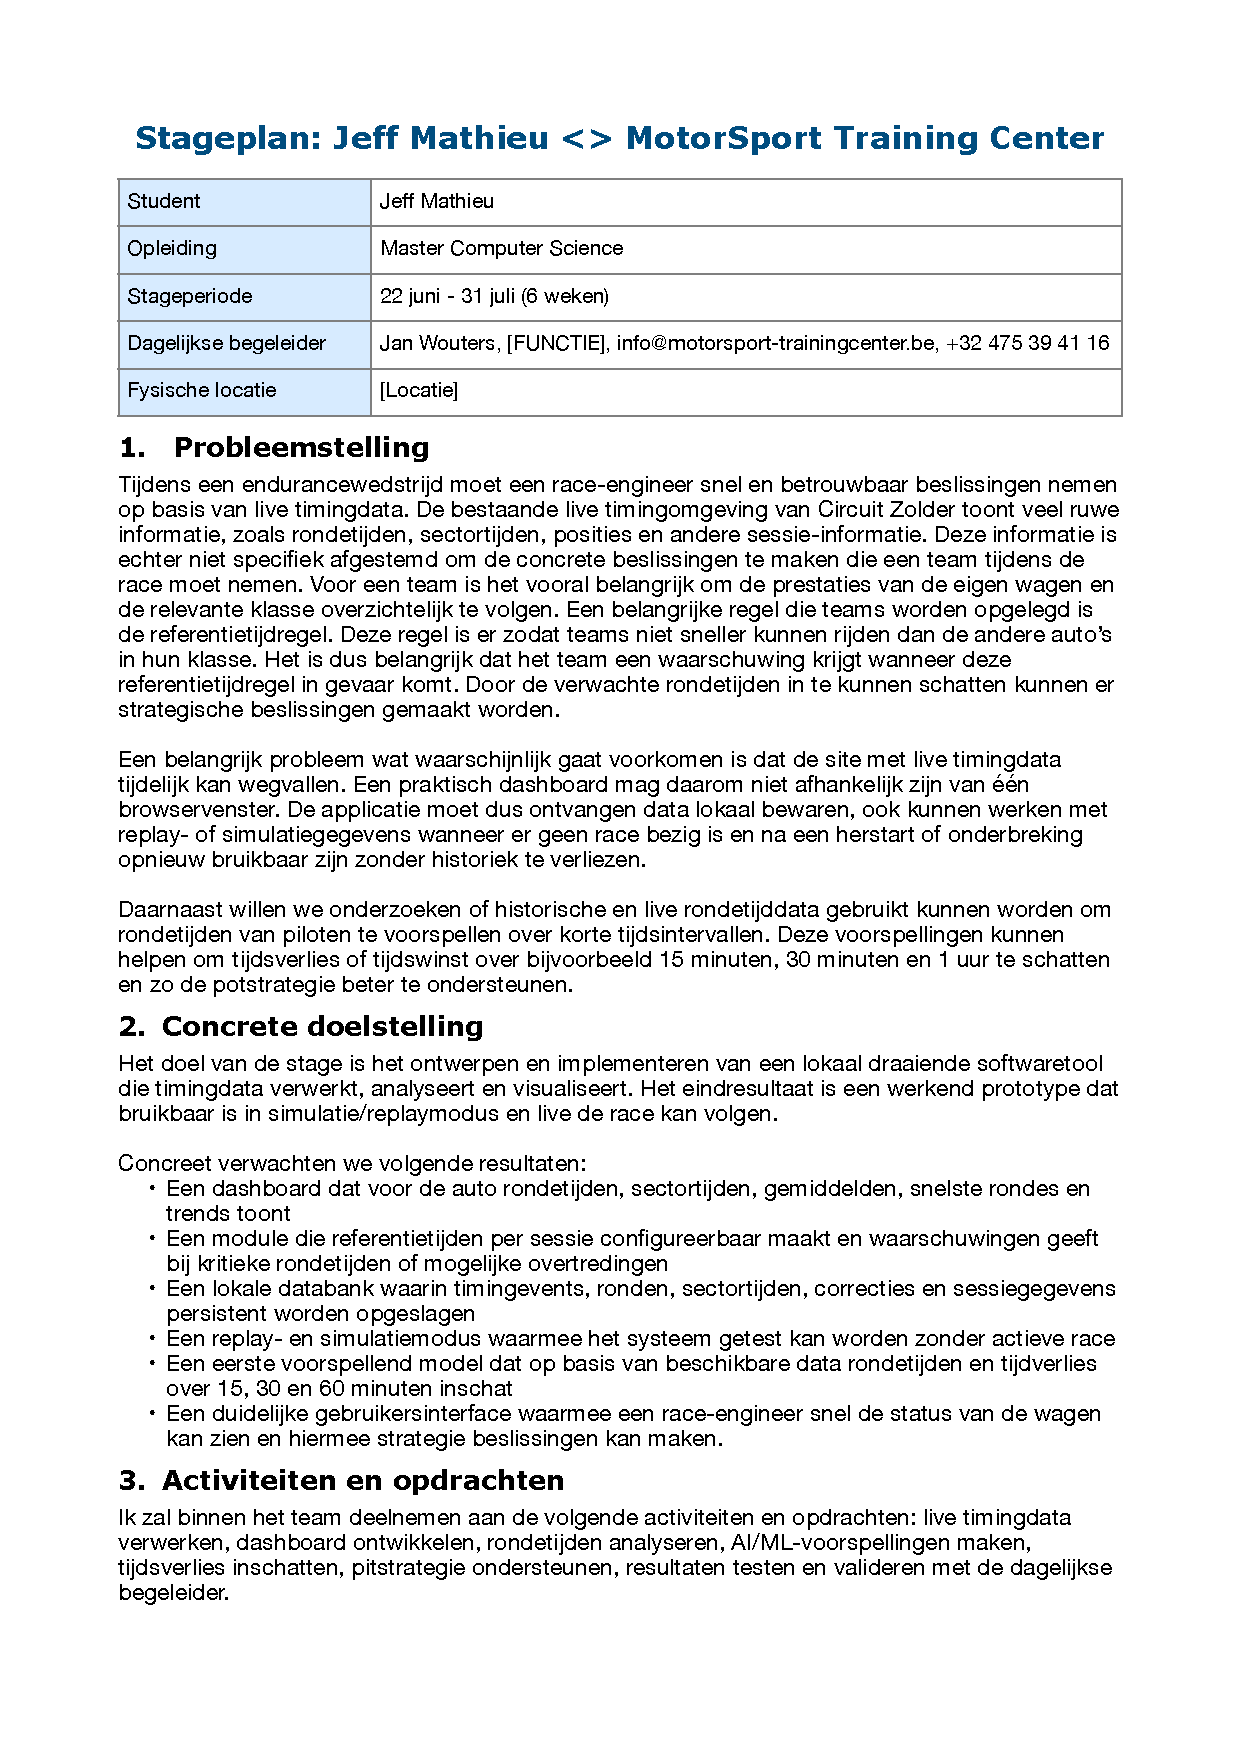
\includepdf[pages=-,pagecommand={}]{appendices/stageplan_Jeff_Mathieu.pdf}

\chapter{Competenties die ik verwachtte te verbeteren}
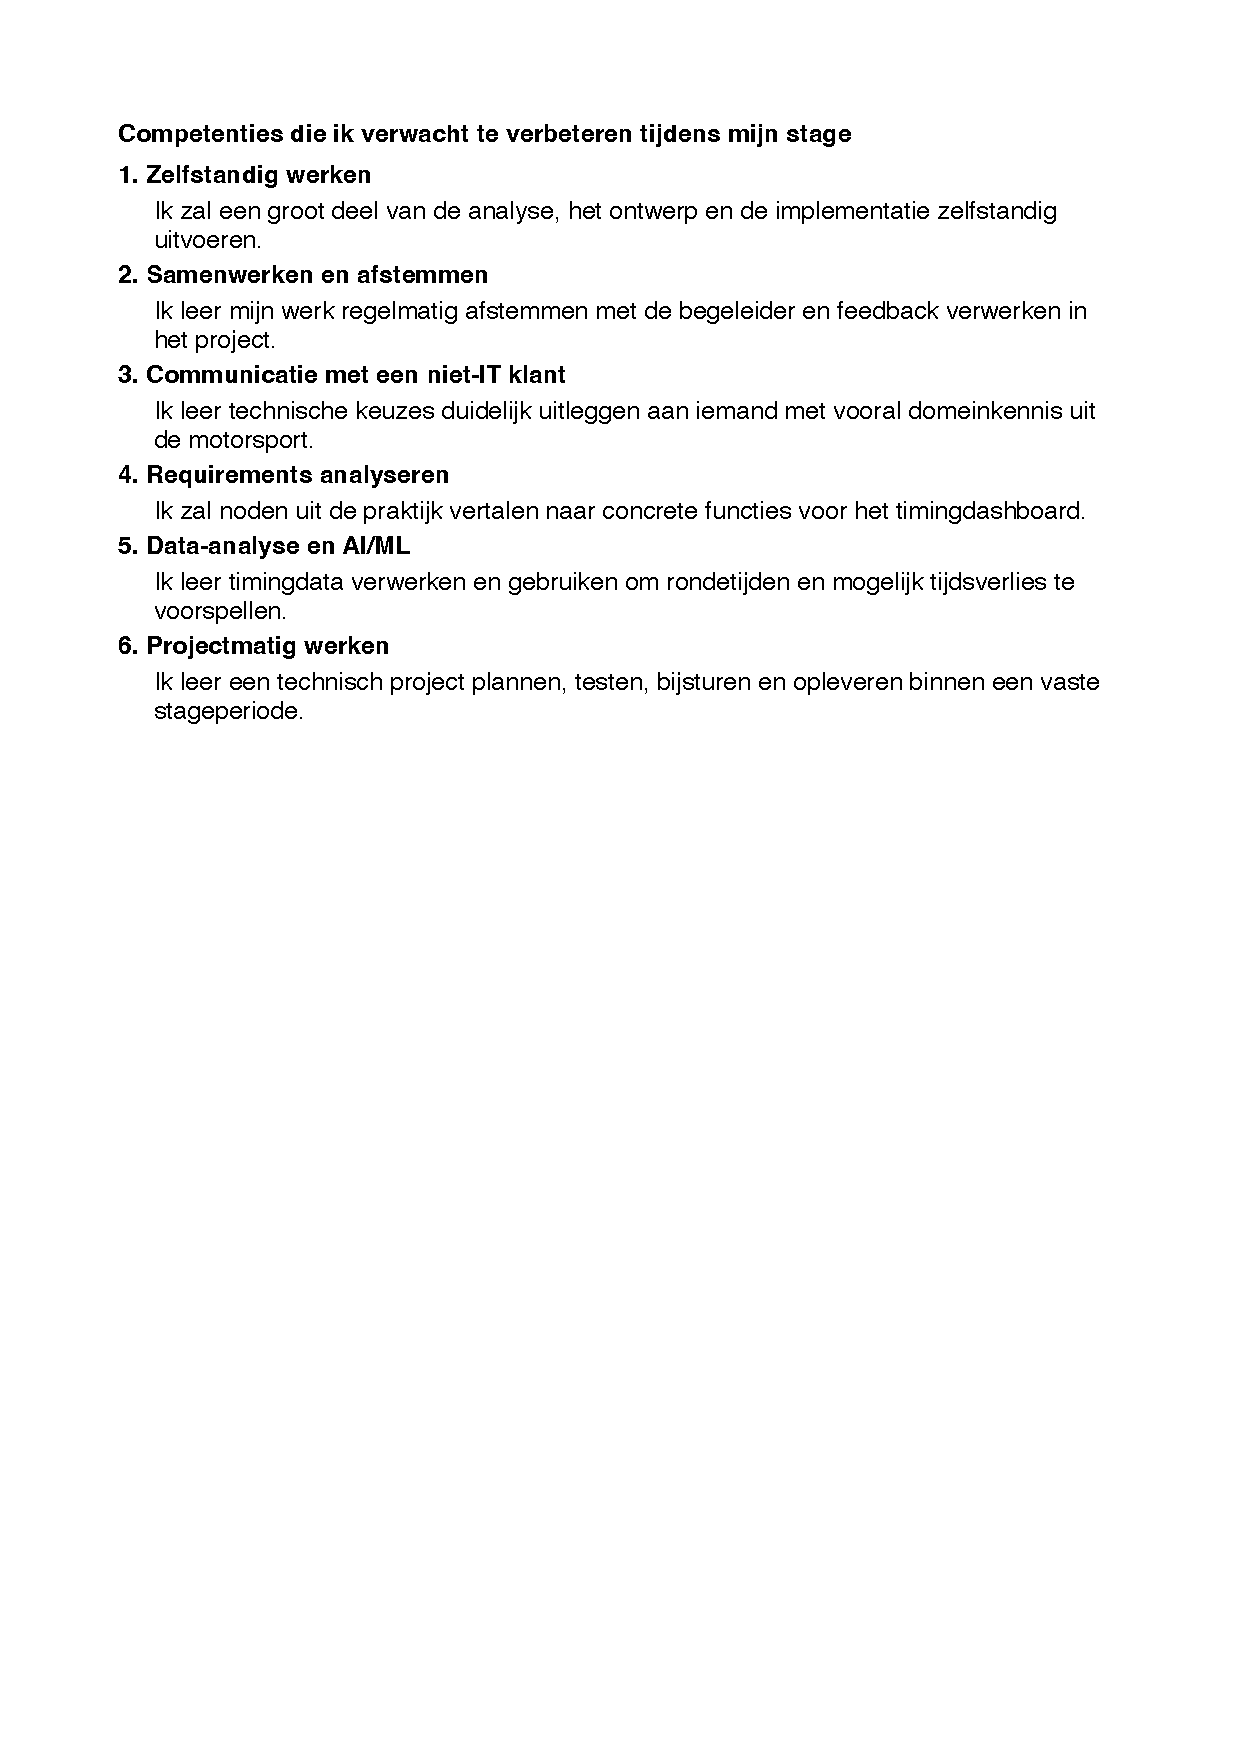
\includepdf[pages=-,pagecommand={}]{appendices/competenties_Jeff_Mathieu.pdf}

\end{document}
